%%%%%%%%%%%%%%%%%%%%%%%%%%%%%%%%%%%%%%%%%%%%%%%%%%%%%%%%%%%%%%%%%%%%%%%%%%%%%%%%
\section{Supplementary materials}
%%%%%%%%%%%%%%%%%%%%%%%%%%%%%%%%%%%%%%%%%%%%%%%%%%%%%%%%%%%%%%%%%%%%%%%%%%%%%%%%

These supplementary materials show the full pipeline and
added diagnostics for the examples in the main article.

As in the main article, all the figures shown in this section are shown as-is, 
without any aesthetical modifications, with the exception that the arrangement
of the sub-figures (for example, aligning true and twin tree
horiztonally) is done manually.

%%%%%%%%%%%%%%%%%%%%%%%%%%%%%%%%%%%%%%%%%%%%%%%%%%%%%%%%%%%%%%%%%%%%%%%%%%%%%%%%
\subsection{Generative model only}
%%%%%%%%%%%%%%%%%%%%%%%%%%%%%%%%%%%%%%%%%%%%%%%%%%%%%%%%%%%%%%%%%%%%%%%%%%%%%%%%

The code used in this part of the article can be found at 
\url{https://github.com/richelbilderbeek/pirouette_example_1}. 

%%%%%%%%%%%%%%%%%%%%%%%%%%%%%%%%%%%%%%%%%%%%%%%%%%%%%%%%%%%%%%%%%%%%%%%%%%%%%%%%
\begin{figure}[H]
  \centering
  \resizebox {0.8\columnwidth} {!} {
    \begin{tikzpicture}[
      ->,>=stealth',shorten >=1pt,auto,
      node distance=0.25\textheight, 
      semithick
    ]   
    \tikzstyle{every state}=[]
    \node[state, draw=none] (O) [] {
    };   
    \node[state] (A) [right of = O, rectangle] {
      \includegraphics[height=0.2\textheight]{example_1/true_tree.png}
    };   
    \node[state] (B) [below of = A, rectangle] {
      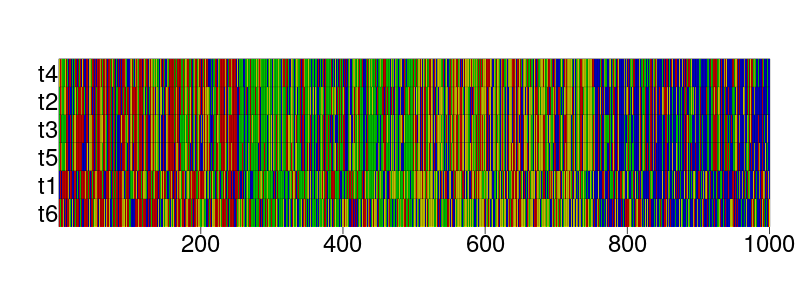
\includegraphics[height=0.2\textheight]{example_1/true_alignment.png}
    };   
    \node[state] (C) [below of = B, rectangle] {
      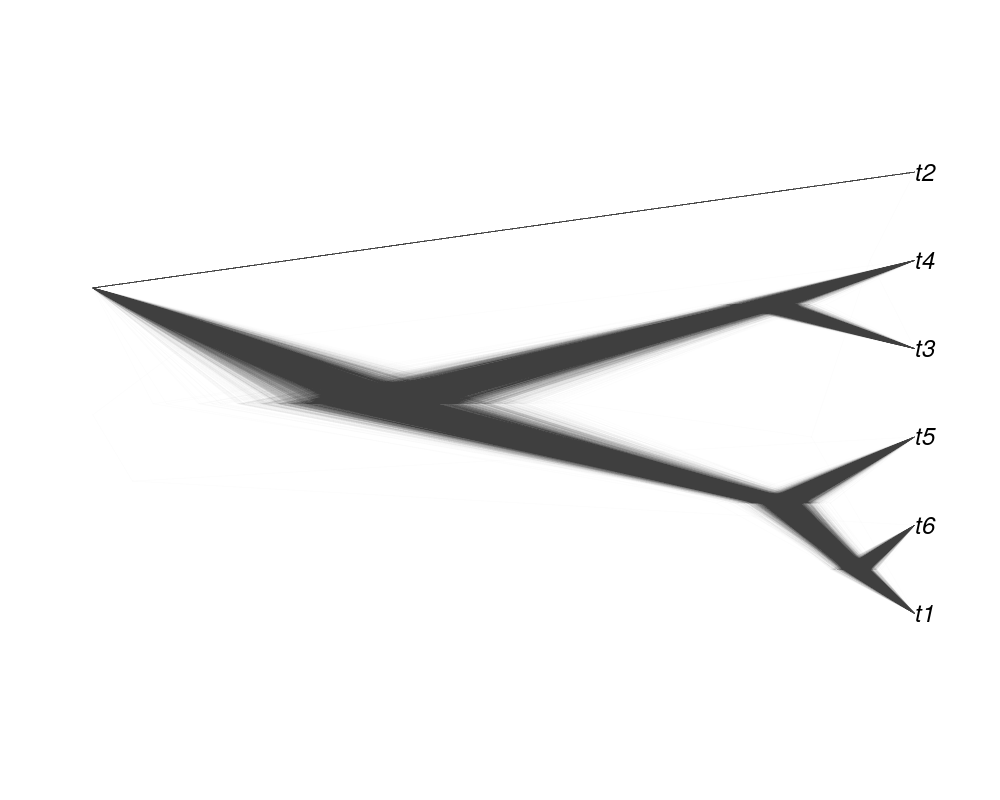
\includegraphics[height=0.2\textheight]{example_1/true_posterior_gen.png}
    };   
    \node[state] (D) [below of = C, rectangle] {
      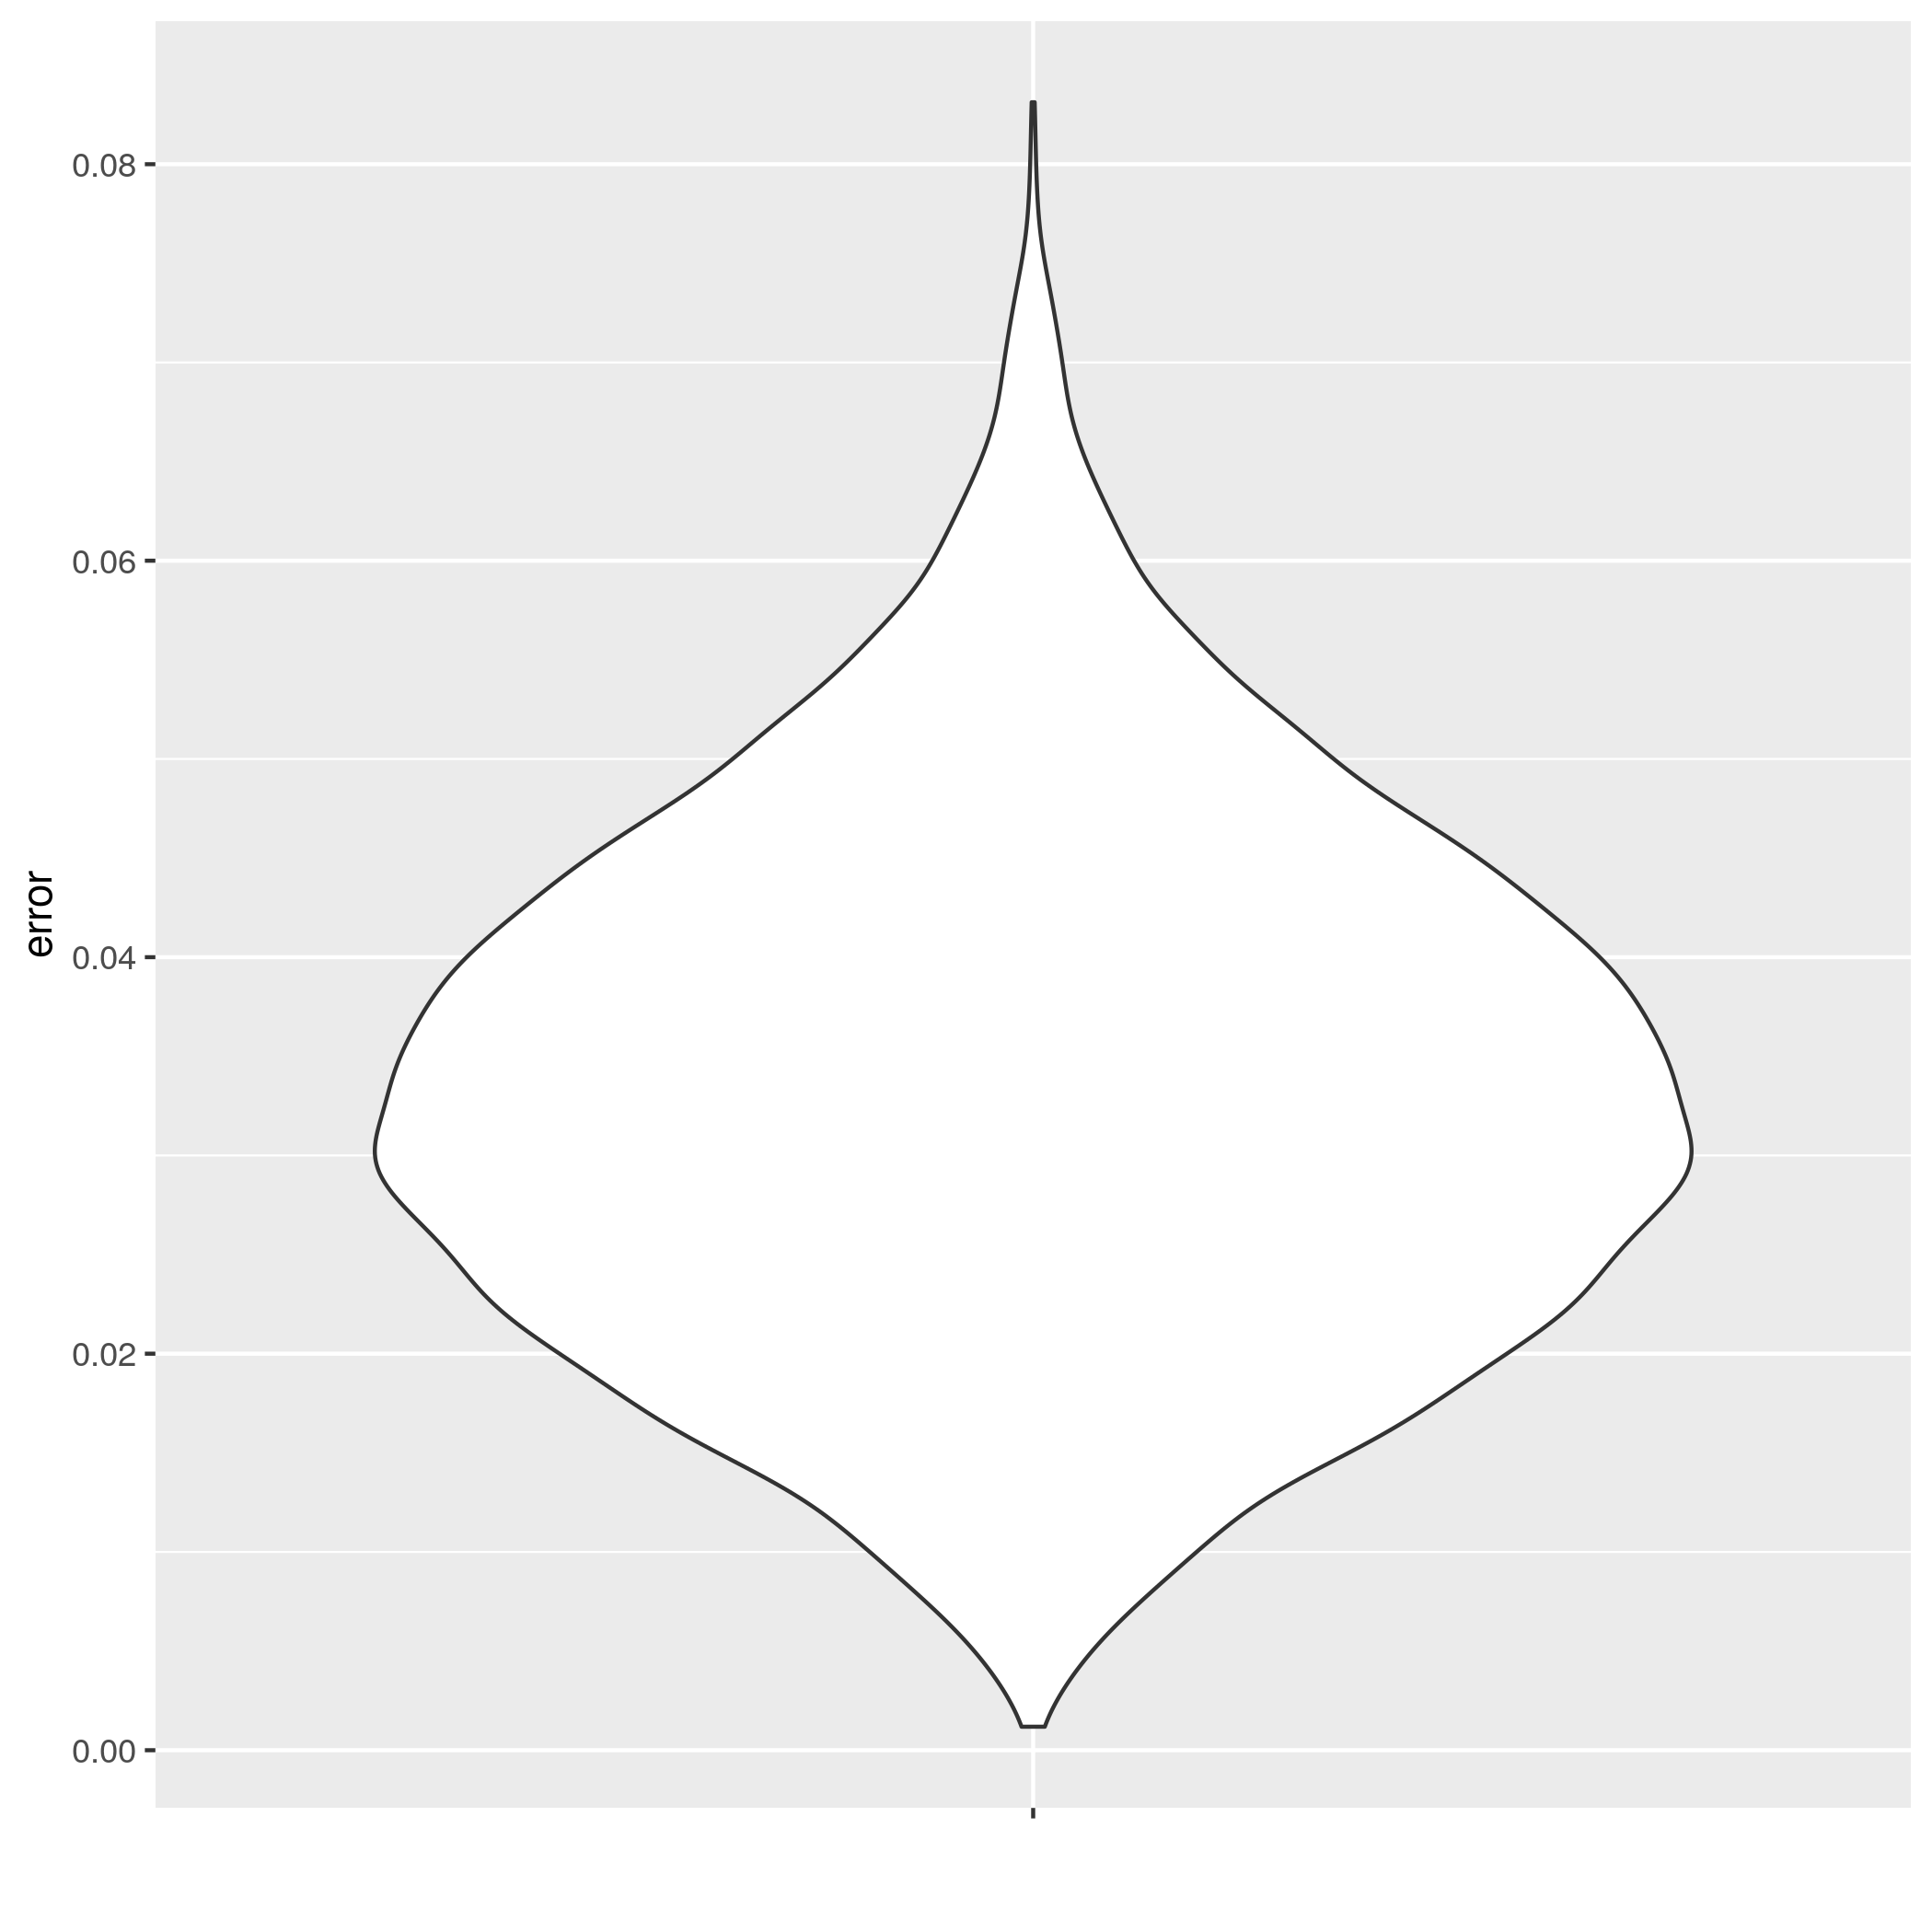
\includegraphics[height=0.2\textheight]{example_1/true_error_violin_gen.png}
    };   
    \path 
      (O) edge [anchor = south] node {} (A)
      (A) edge [anchor = south] node {} (B)
      (B) edge [anchor = south] node {} (C)
      (C) edge [anchor = south] node {} (D)
    ; 
    \end{tikzpicture}
  }
  \label{fig:example_1_full_pipeline}
  \caption{Generative model only: full pipeline}
\end{figure}
%%%%%%%%%%%%%%%%%%%%%%%%%%%%%%%%%%%%%%%%%%%%%%%%%%%%%%%%%%%%%%%%%%%%%%%%%%%%%%%%

%%%%%%%%%%%%%%%%%%%%%%%%%%%%%%%%%%%%%%%%%%%%%%%%%%%%%%%%%%%%%%%%%%%%%%%%%%%%%%%%

\input{example_1/esses_gen.latex}

%%%%%%%%%%%%%%%%%%%%%%%%%%%%%%%%%%%%%%%%%%%%%%%%%%%%%%%%%%%%%%%%%%%%%%%%%%%%%%%%



%%%%%%%%%%%%%%%%%%%%%%%%%%%%%%%%%%%%%%%%%%%%%%%%%%%%%%%%%%%%%%%%%%%%%%%%%%%%%%%%
\subsection{Comparing to other candidate models}
%%%%%%%%%%%%%%%%%%%%%%%%%%%%%%%%%%%%%%%%%%%%%%%%%%%%%%%%%%%%%%%%%%%%%%%%%%%%%%%%

The code used in this part of the article can be found at 
\url{https://github.com/richelbilderbeek/pirouette_example_2}. 

%%%%%%%%%%%%%%%%%%%%%%%%%%%%%%%%%%%%%%%%%%%%%%%%%%%%%%%%%%%%%%%%%%%%%%%%%%%%%%%%
\begin{figure}[H]
  \centering
  \resizebox {0.8\columnwidth} {!} {
    \begin{tikzpicture}[
      ->,>=stealth',shorten >=1pt,auto,
      node distance=0.7\textheight, 
      semithick
    ]   
    \tikzstyle{every state}=[]
    \node[state, draw=none] (O) [] {
    };   
    \node[state] (A) [right of = O, rectangle] {
      \includegraphics[height=0.5\textheight]{example_2/true_tree.png}
    };   
    \node[state] (B) [below of = A, rectangle] {
      \includegraphics[height=0.5\textheight]{example_2/true_alignment.png}
    };   
    \node[state] (CG) [below of = B, rectangle] {
      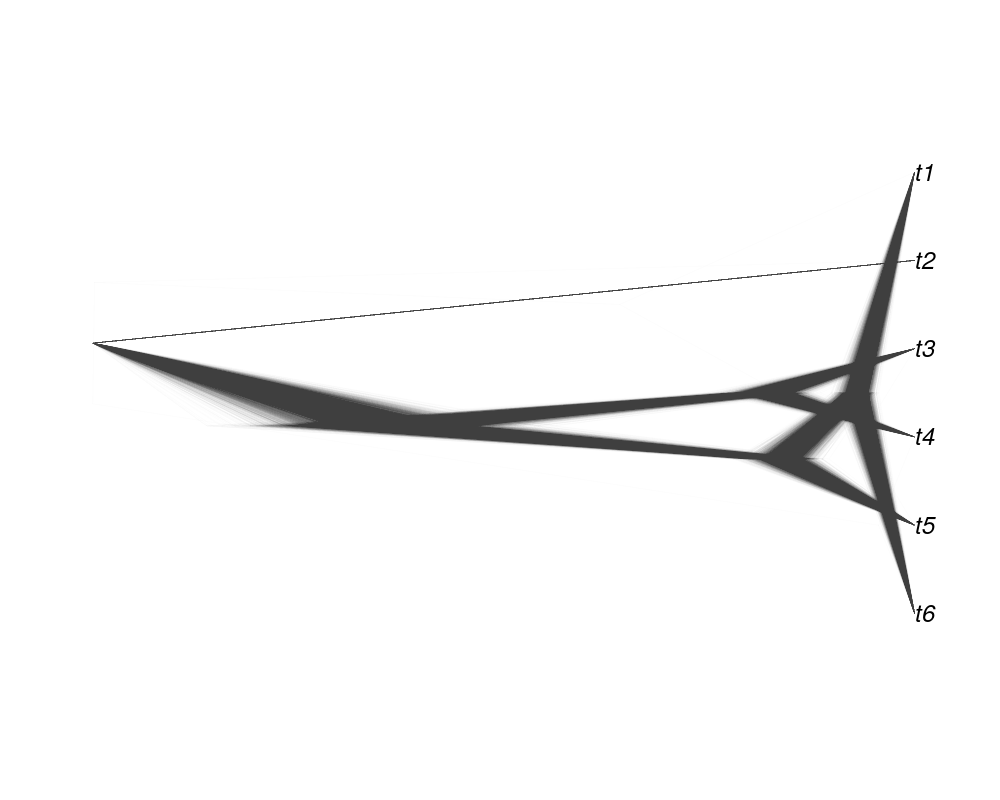
\includegraphics[height=0.45\textheight]{example_2/true_posterior_gen.png}
    };   
    \node[state] (DG) [below of = CG, rectangle] {
      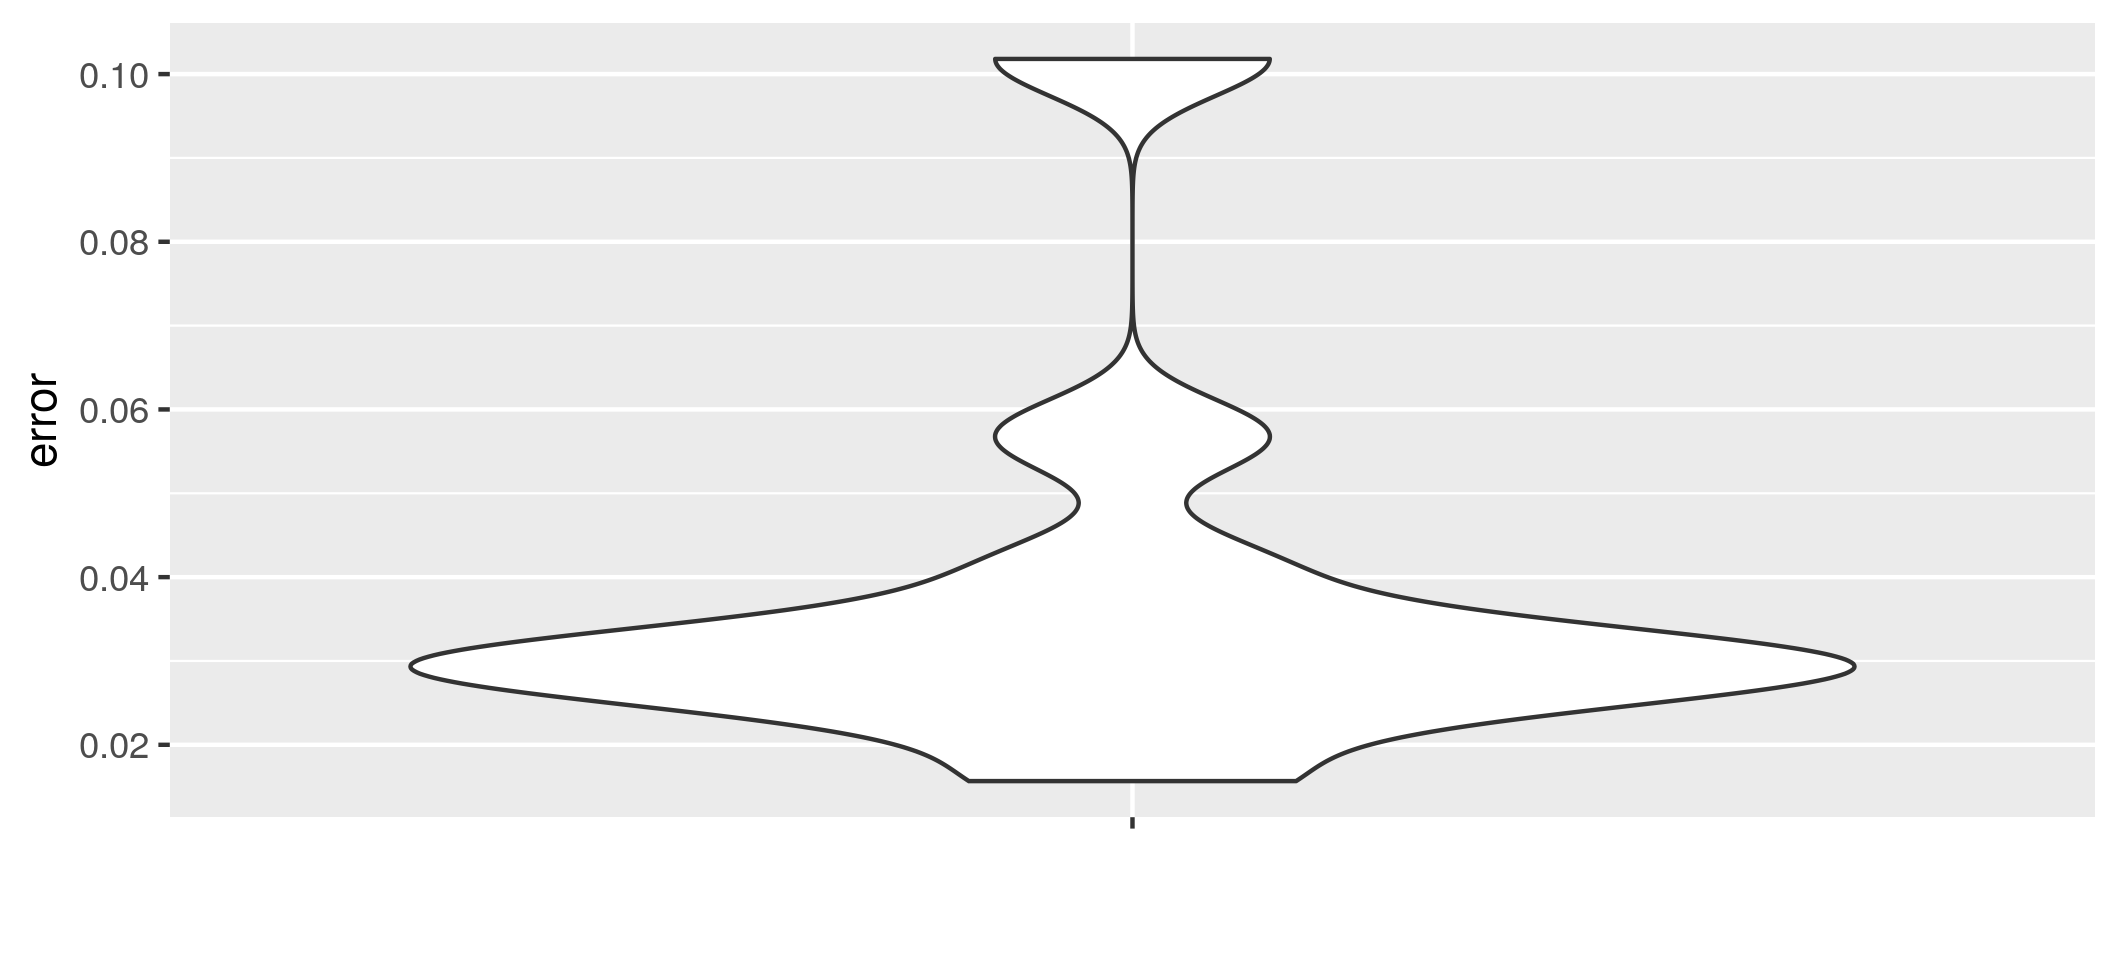
\includegraphics[height=0.3\textheight]{example_2/true_error_violin_gen.png}
    };   
    \node[state] (CB) [right of = CG, rectangle] {
      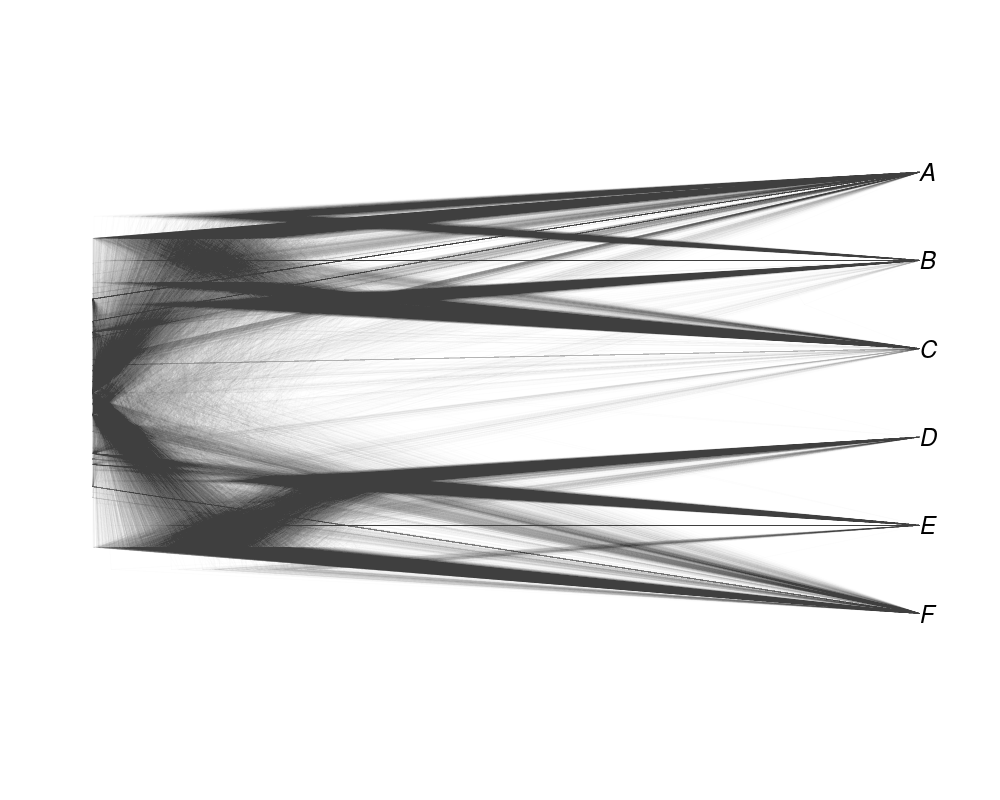
\includegraphics[height=0.45\textheight]{example_2/true_posterior_best.png}
    };   
    \node[state] (DB) [right of = DG, rectangle] {
      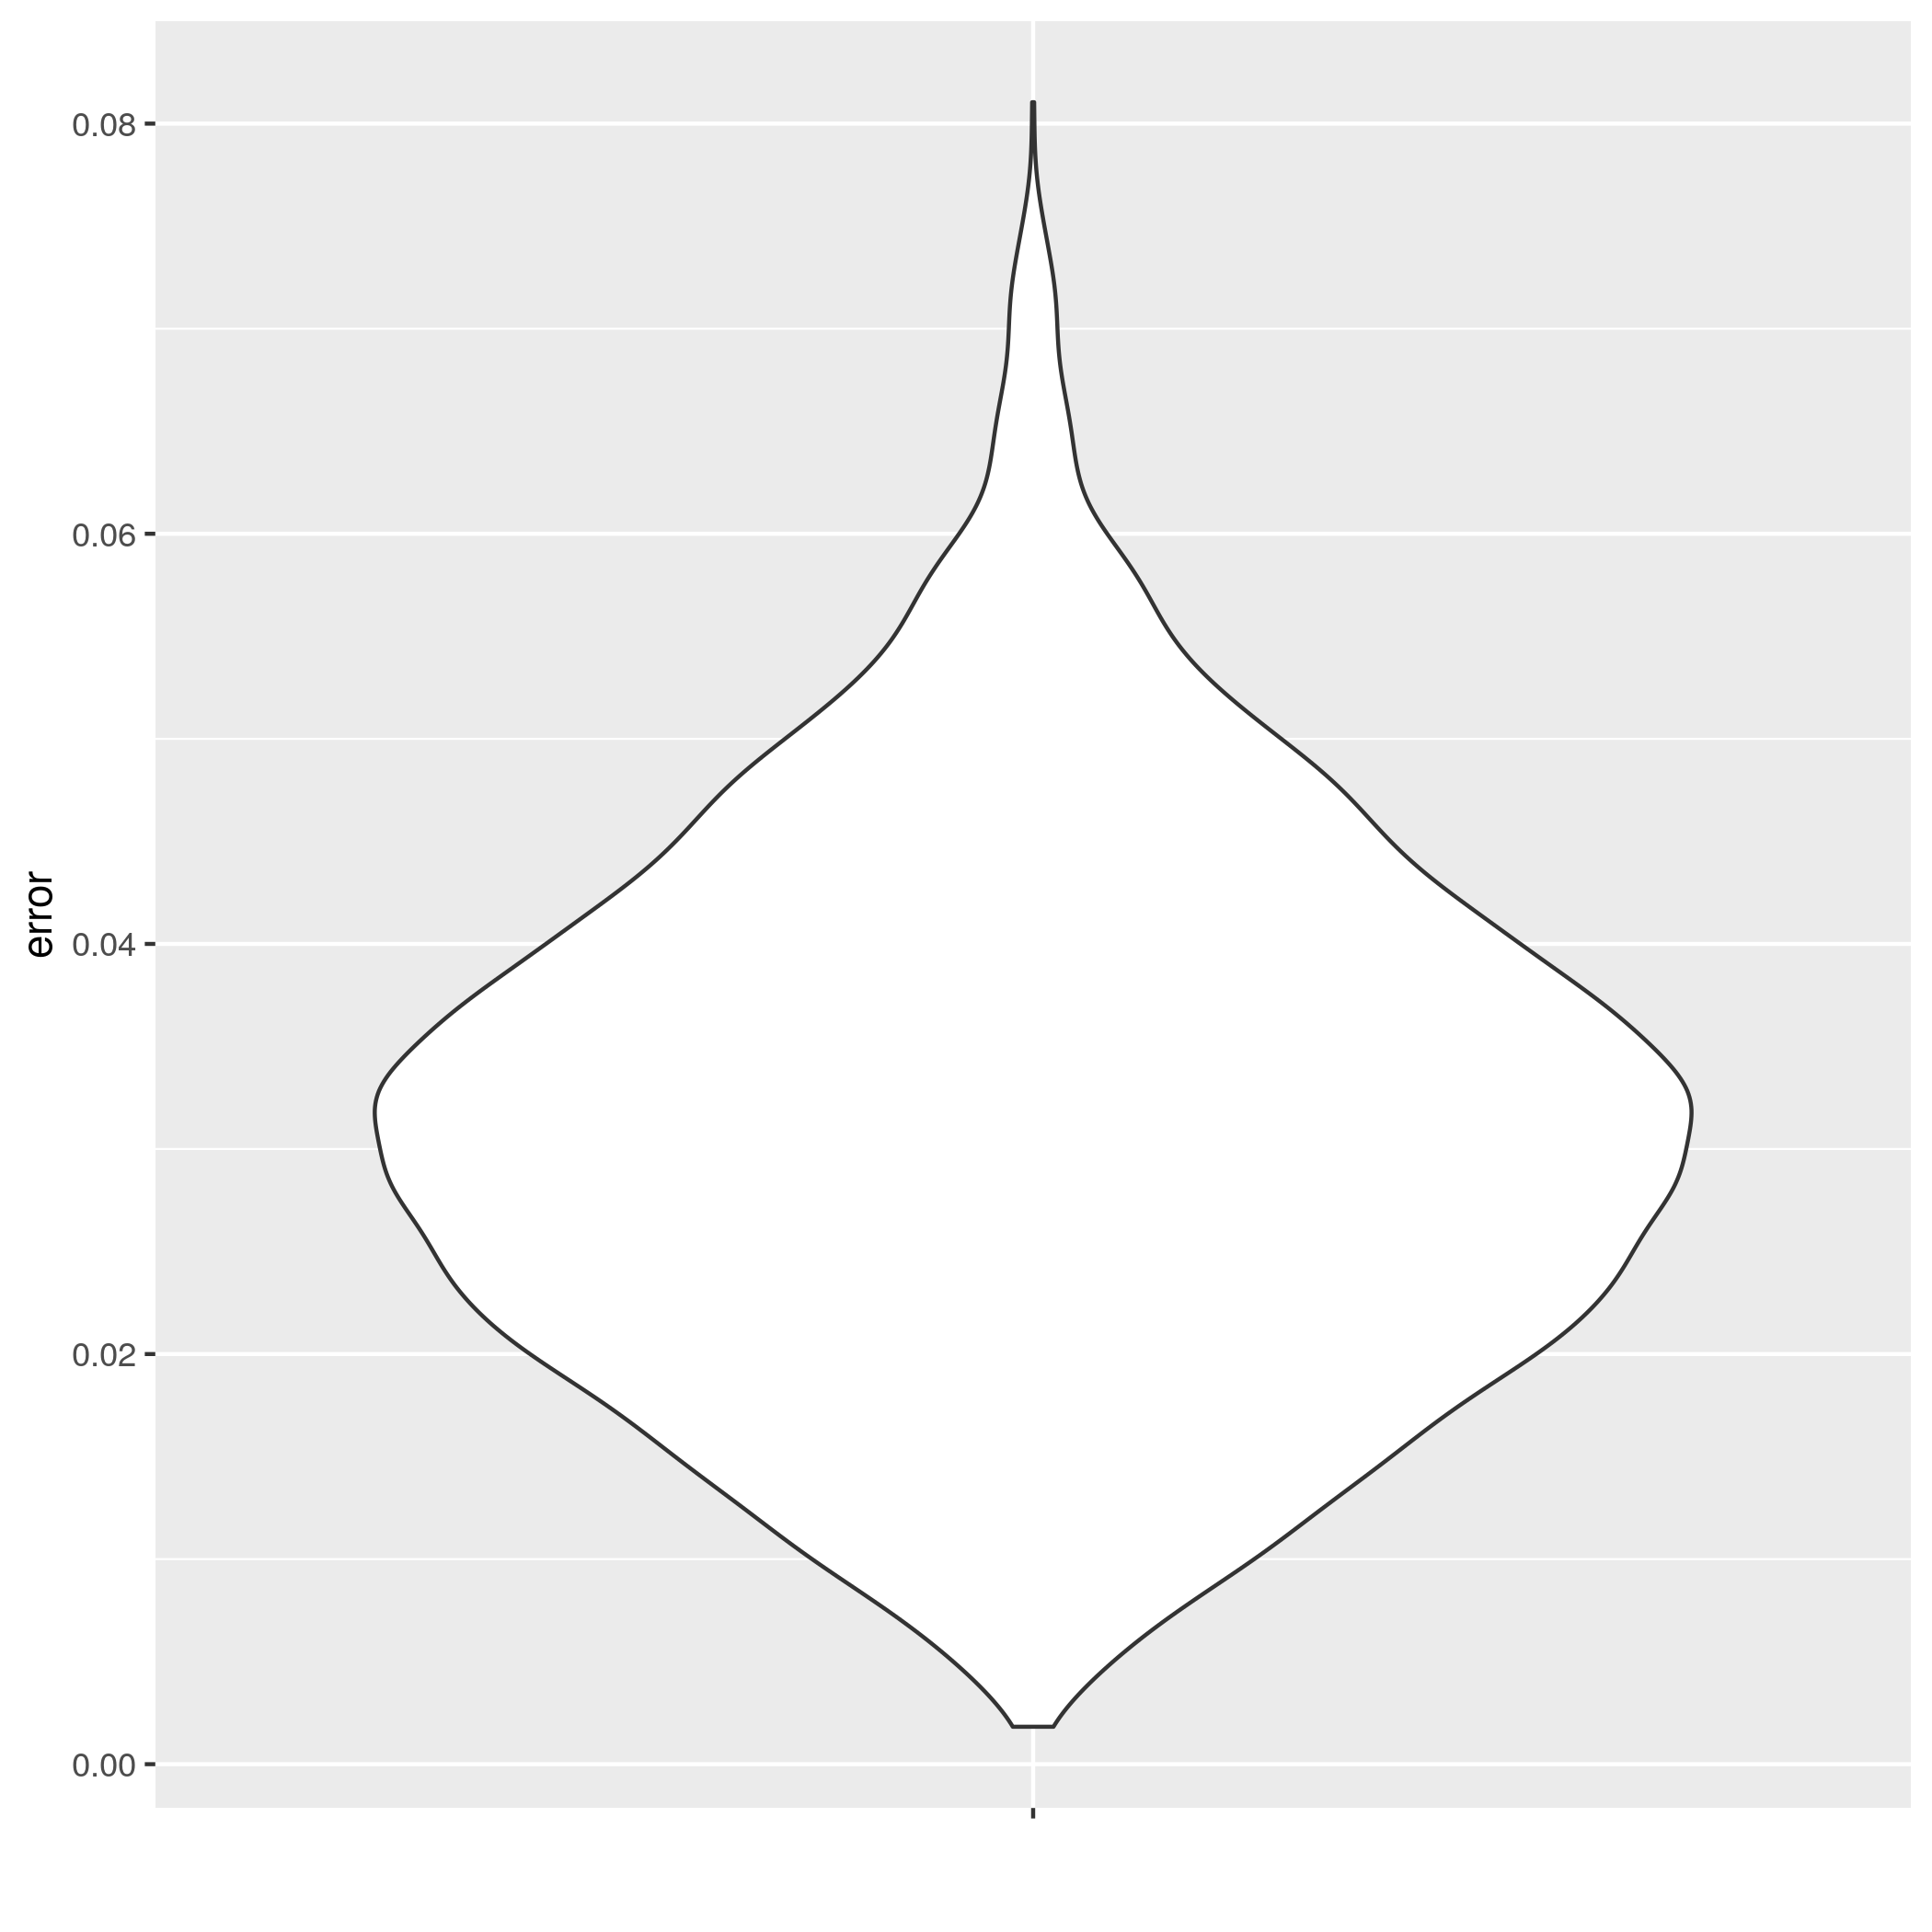
\includegraphics[height=0.3\textheight]{example_2/true_error_violin_best.png}
    };   
    \path 
      (O) edge [anchor = south] node {} (A)
      (A) edge [anchor = south] node {} (B)
      (B) edge [anchor = south] node {} (CG)
      (CG) edge [anchor = south] node {} (DG)
      (B) edge [anchor = south] node {} (CB)
      (CB) edge [anchor = south] node {} (DB)
    ; 
    \end{tikzpicture}
  }
  \label{fig:example_2_full_pipeline}
  \caption{Comparing to other candidate models: full pipeline}
\end{figure}
%%%%%%%%%%%%%%%%%%%%%%%%%%%%%%%%%%%%%%%%%%%%%%%%%%%%%%%%%%%%%%%%%%%%%%%%%%%%%%%%

\input{example_2/esses_gen.latex}

\input{example_2/esses_best.latex}

\input{example_2/evidence_true.latex}

%%%%%%%%%%%%%%%%%%%%%%%%%%%%%%%%%%%%%%%%%%%%%%%%%%%%%%%%%%%%%%%%%%%%%%%%%%%%%%%%
\subsection{Comparing to background noise}
%%%%%%%%%%%%%%%%%%%%%%%%%%%%%%%%%%%%%%%%%%%%%%%%%%%%%%%%%%%%%%%%%%%%%%%%%%%%%%%%

The code used in this part of the article can be found at 
\url{https://github.com/richelbilderbeek/pirouette_example_3}.

%%%%%%%%%%%%%%%%%%%%%%%%%%%%%%%%%%%%%%%%%%%%%%%%%%%%%%%%%%%%%%%%%%%%%%%%%%%%%%%%
\begin{figure}[H]
  \centering
  \resizebox {1.0\columnwidth} {!} {
    \begin{tikzpicture}[
      ->,>=stealth',shorten >=1pt,auto,
      node distance=0.5\textheight, 
      semithick
    ]   
    \tikzstyle{every state}=[]
    \node[state, draw=none] (O) [] {
    };   
    \node[state] (A) [right of = O, rectangle] {
      \includegraphics[height=0.4\textheight]{example_3/true_tree.png}
    };   
    \node[state] (B) [below of = A, rectangle] {
      \includegraphics[height=0.25\textheight]{example_3/true_alignment.png}
    };   
    \node[state] (CG) [below of = B, rectangle] {
      
\includegraphics[height=0.3\textheight]{example_3/true_posterior_gen.png}
    };   
    \node[state] (DG) [below of = CG, rectangle] {
      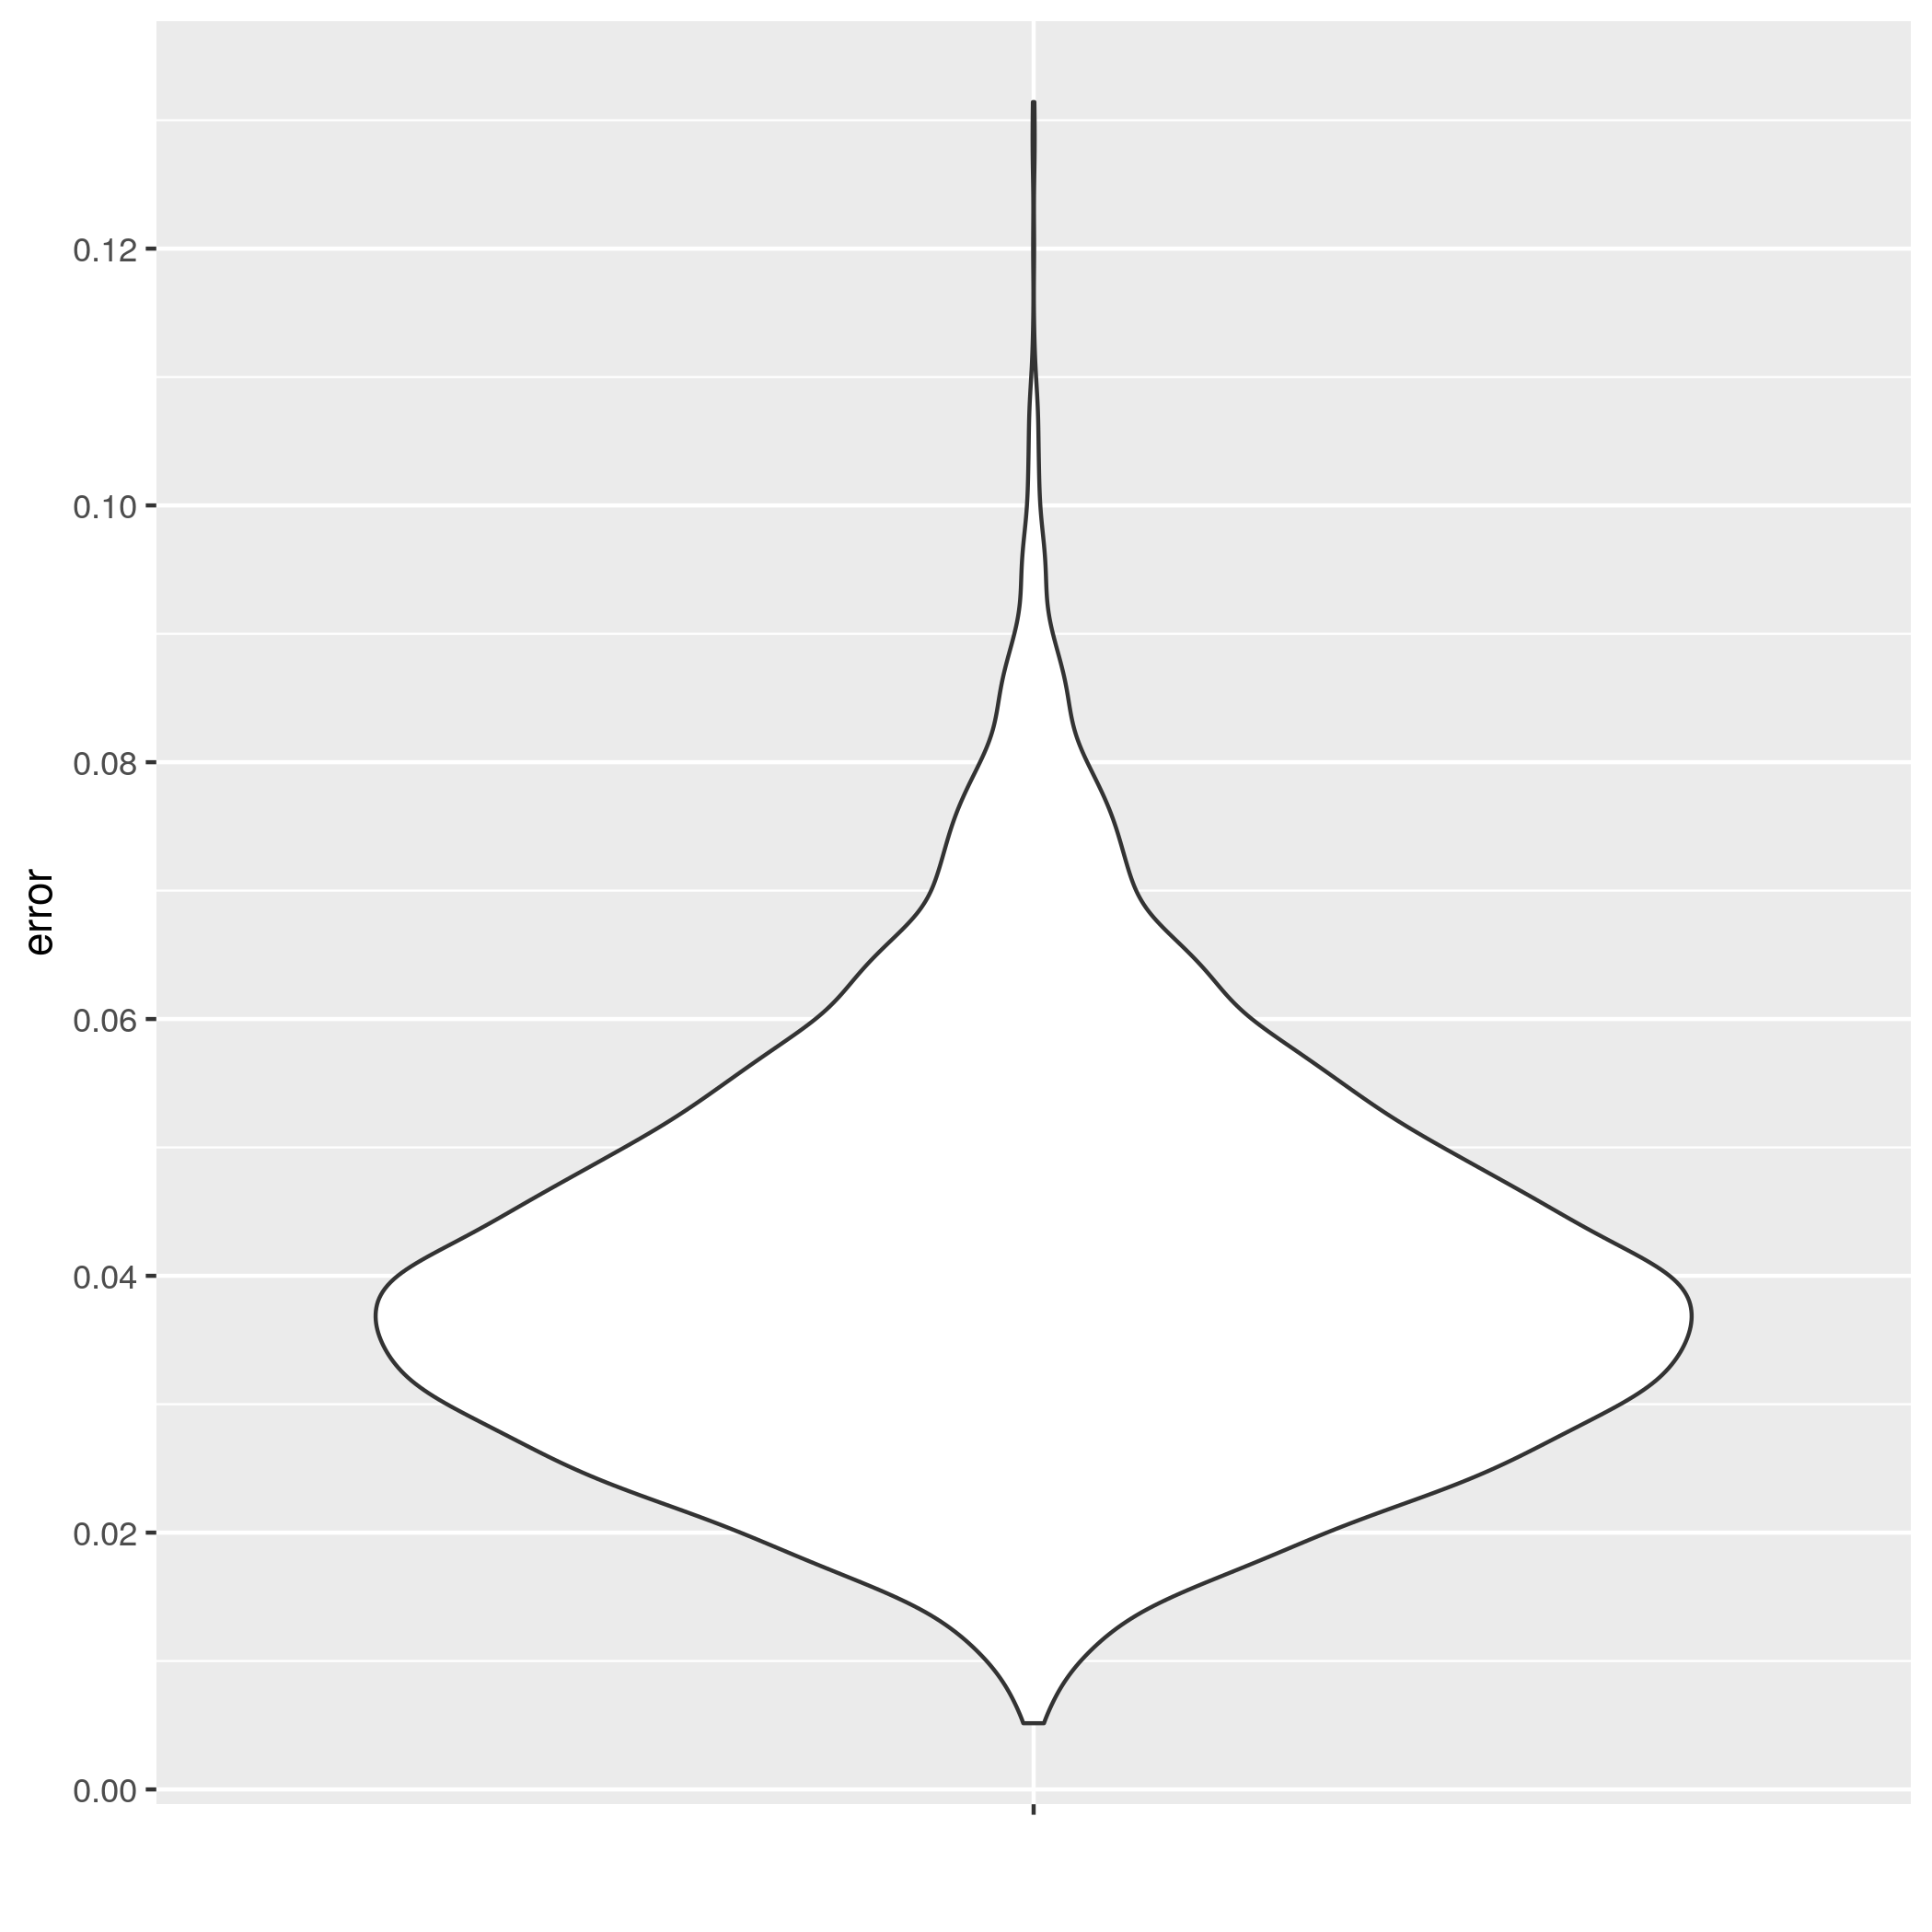
\includegraphics[height=0.3\textheight]{example_3/true_error_violin_gen.png}
    };   
    \node[state] (CB) [right of = CG, rectangle] {
      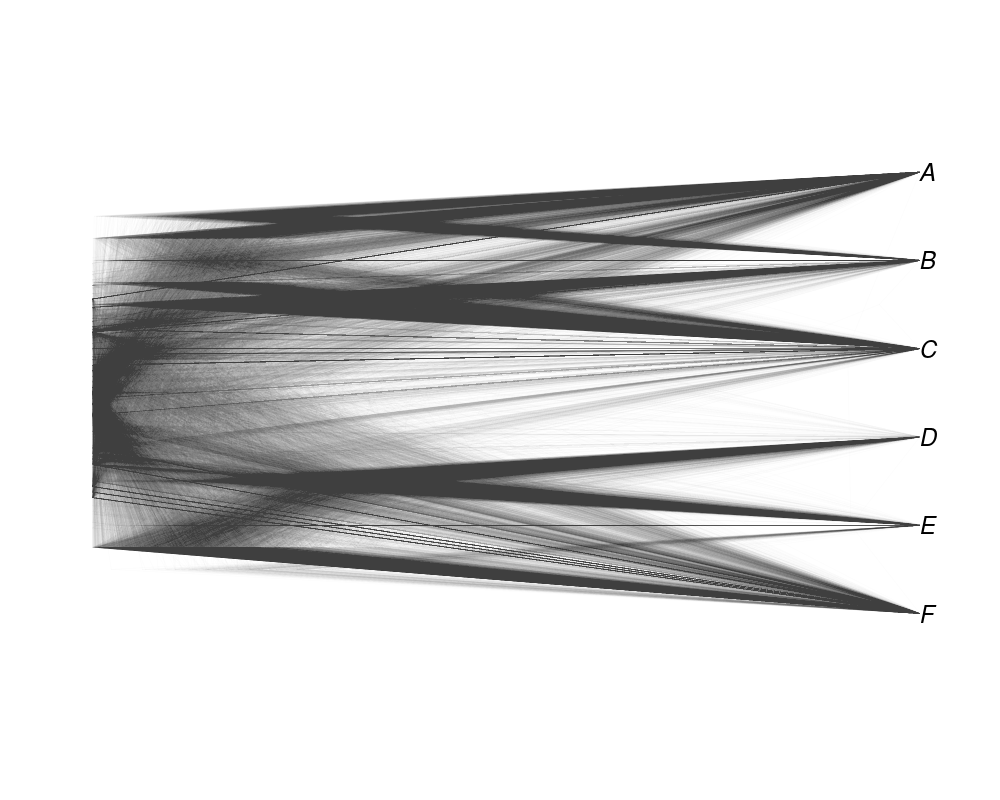
\includegraphics[height=0.3\textheight]{example_3/true_posterior_best.png}
    };   
    \node[state] (DB) [below of = CB, rectangle] {
      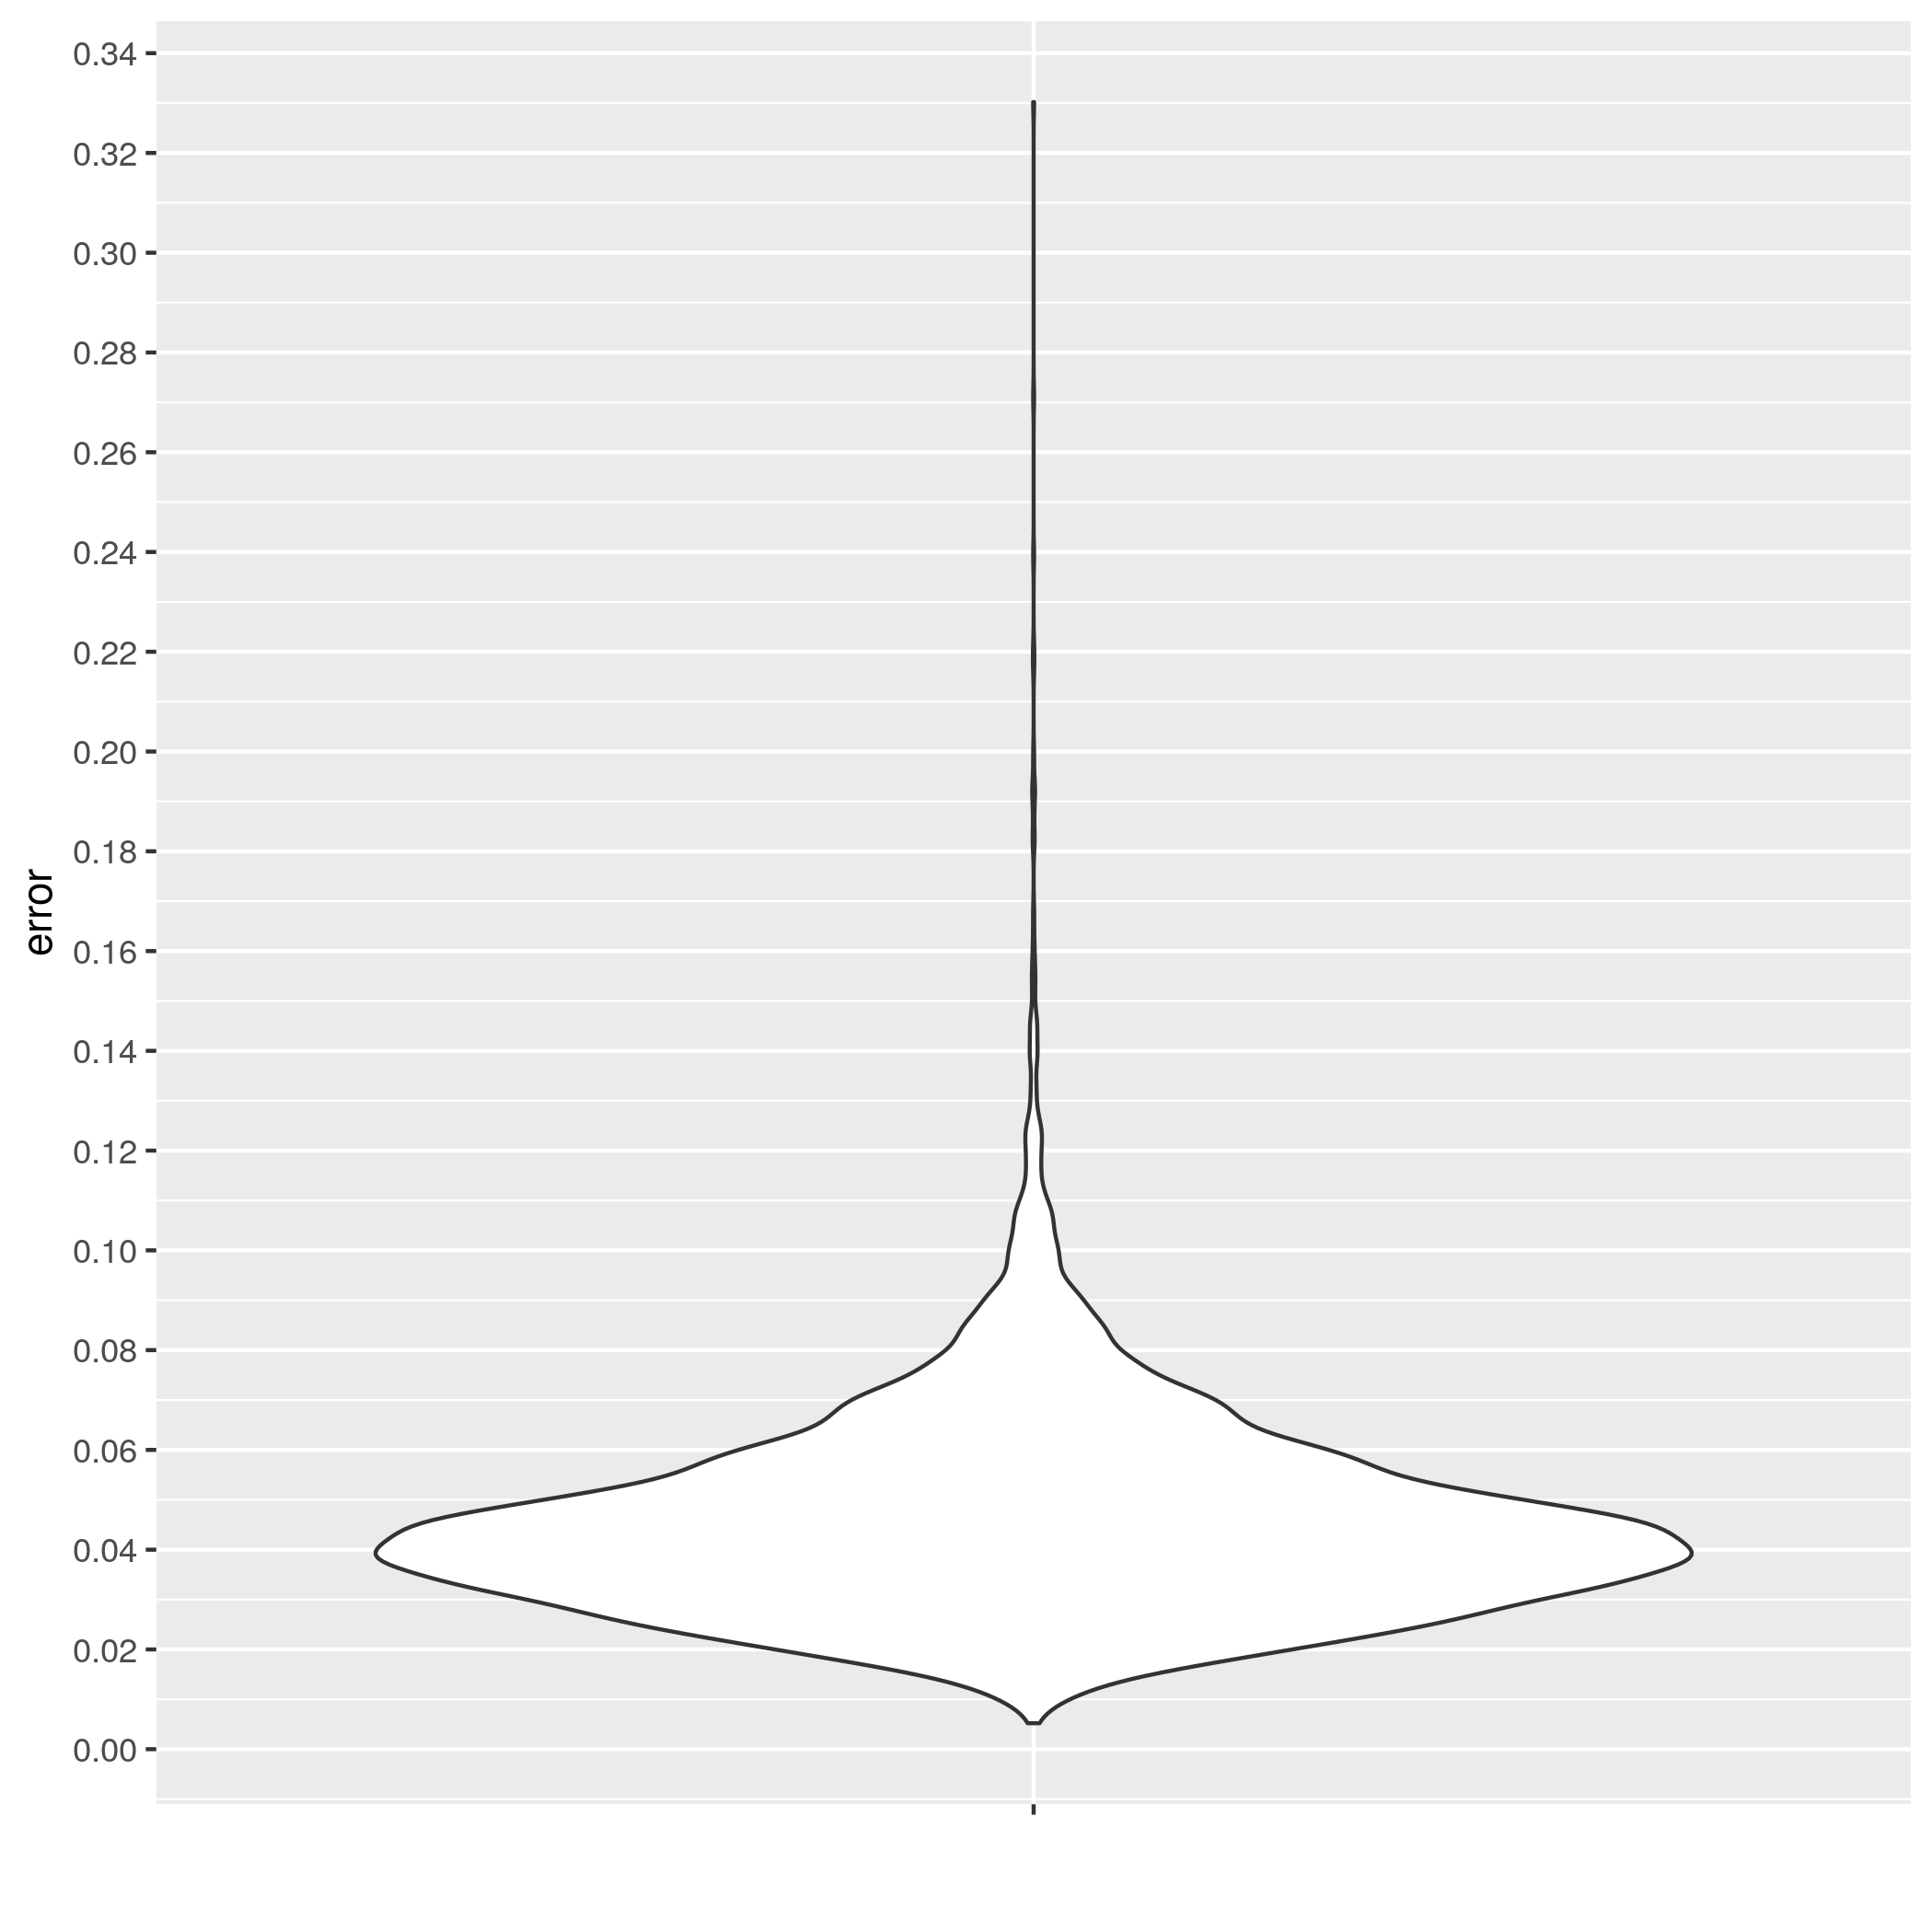
\includegraphics[height=0.3\textheight]{example_3/true_error_violin_best.png}
    };   
    \node[state] (AT) [right of = A, rectangle, node distance=0.8\textheight] {
      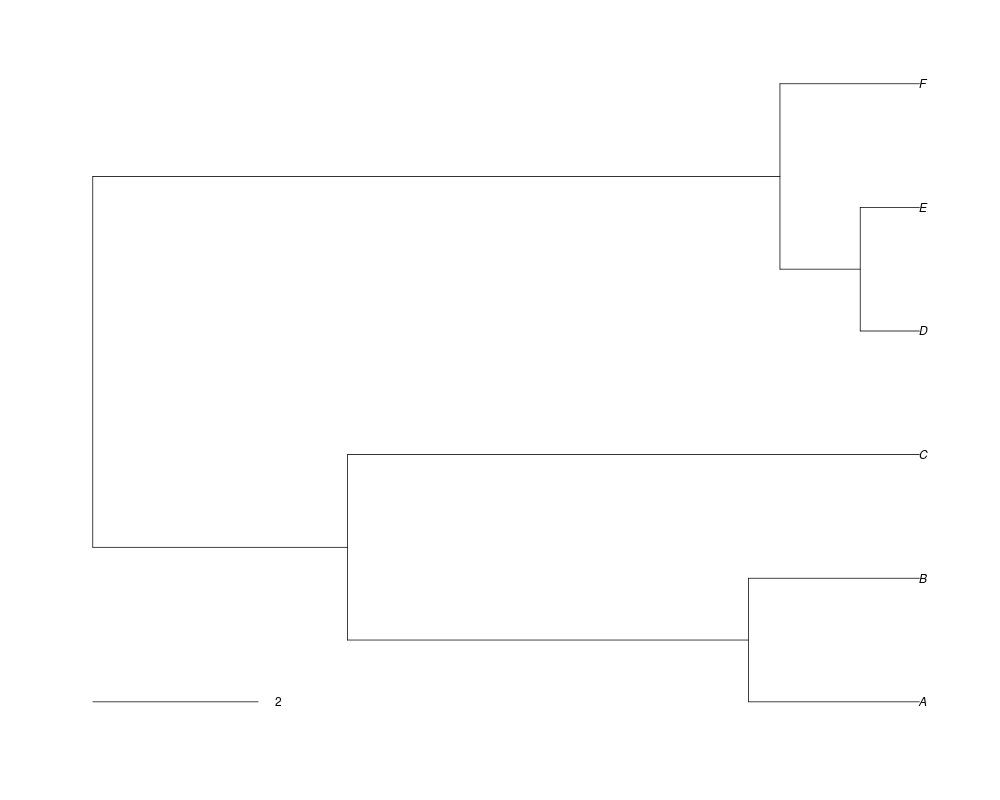
\includegraphics[height=0.4\textheight]{example_3/twin_tree.png}
    };   
    \node[state] (BT) [below of = AT, rectangle] {
      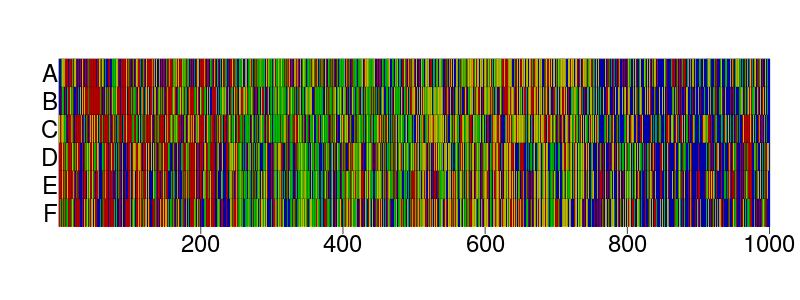
\includegraphics[height=0.25\textheight]{example_3/twin_alignment.png}
    };   
    \node[state] (CTG) [right of = CB, rectangle] {
      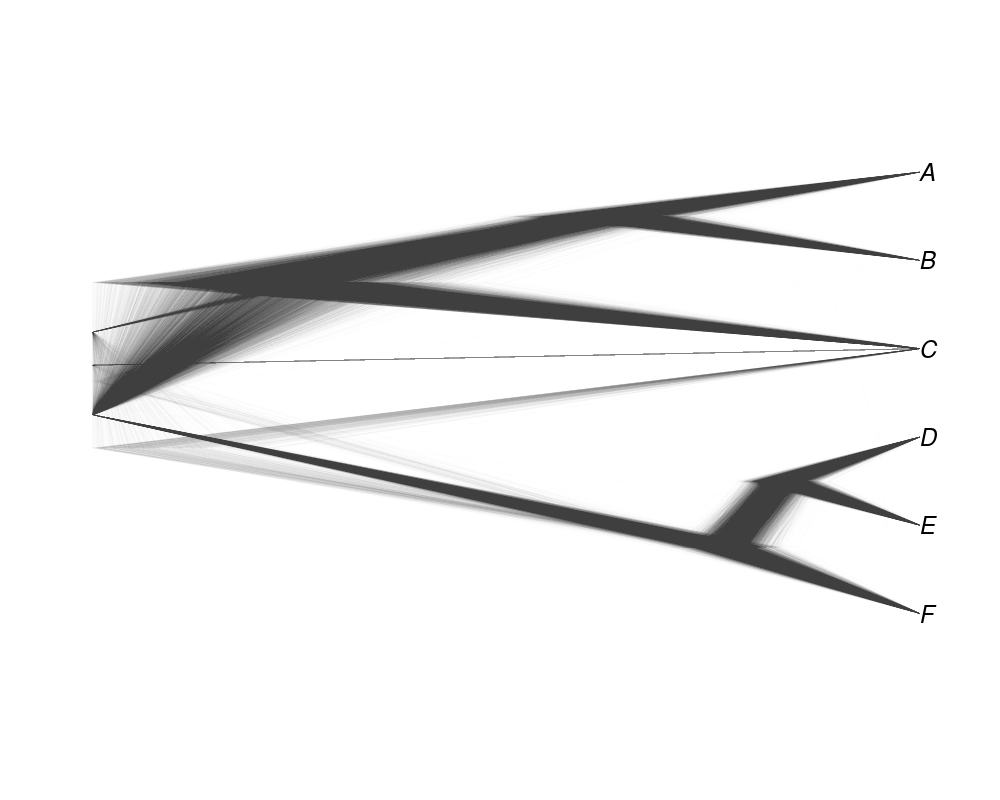
\includegraphics[height=0.3\textheight]{example_3/twin_posterior_gen.png}
    };   
    \node[state] (DTG) [below of = CTG, rectangle] {
      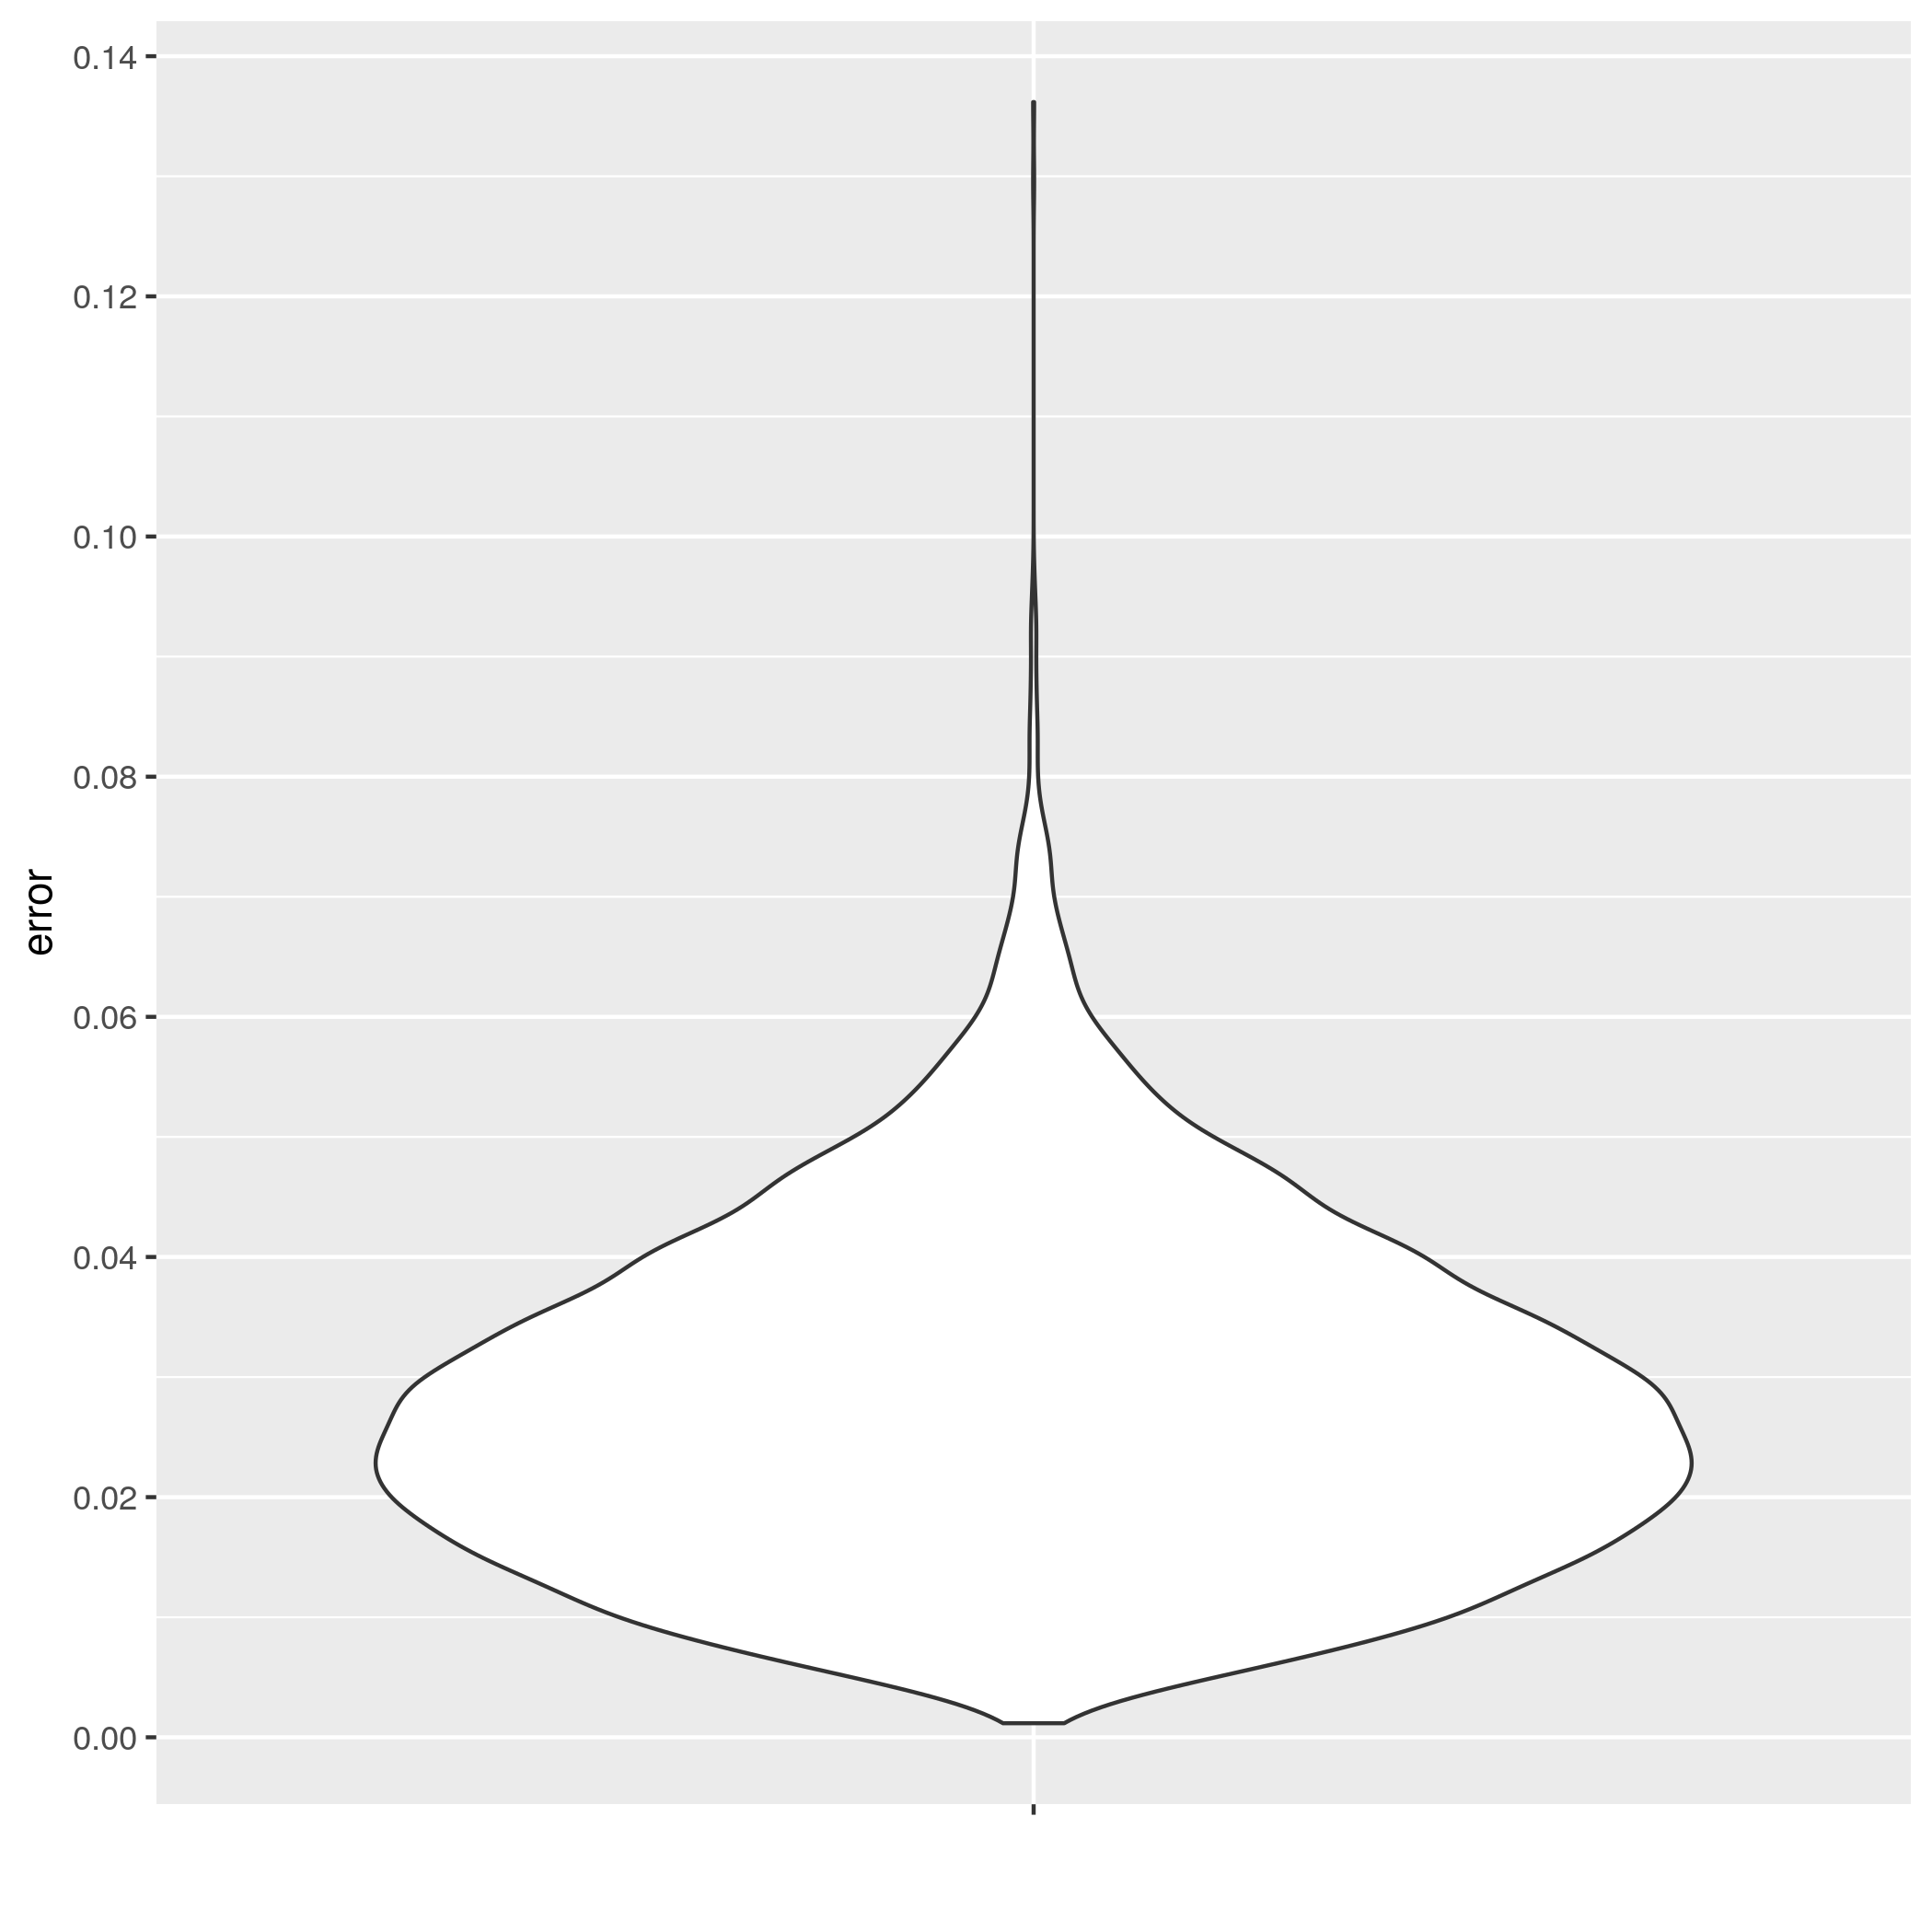
\includegraphics[height=0.3\textheight]{example_3/twin_error_violin_gen.png}
    };   
    \node[state] (CTB) [right of = CTG, rectangle] {
      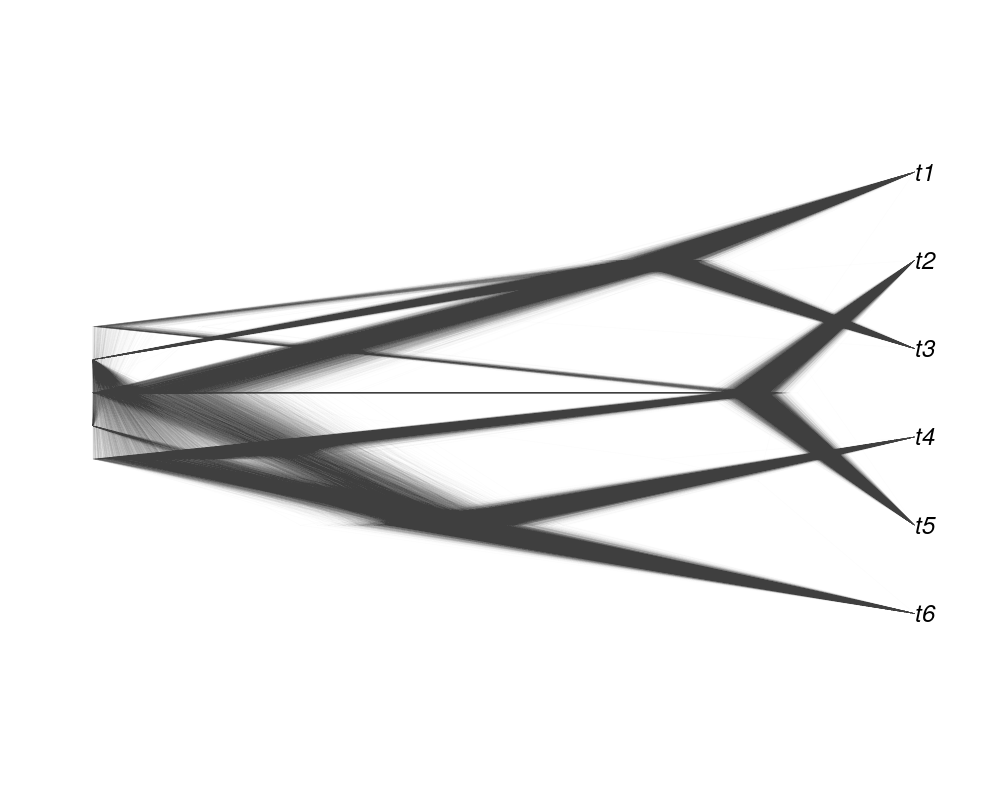
\includegraphics[height=0.3\textheight]{example_3/twin_posterior_best.png}
    };   
    \node[state] (DTB) [below of = CTB, rectangle] {
      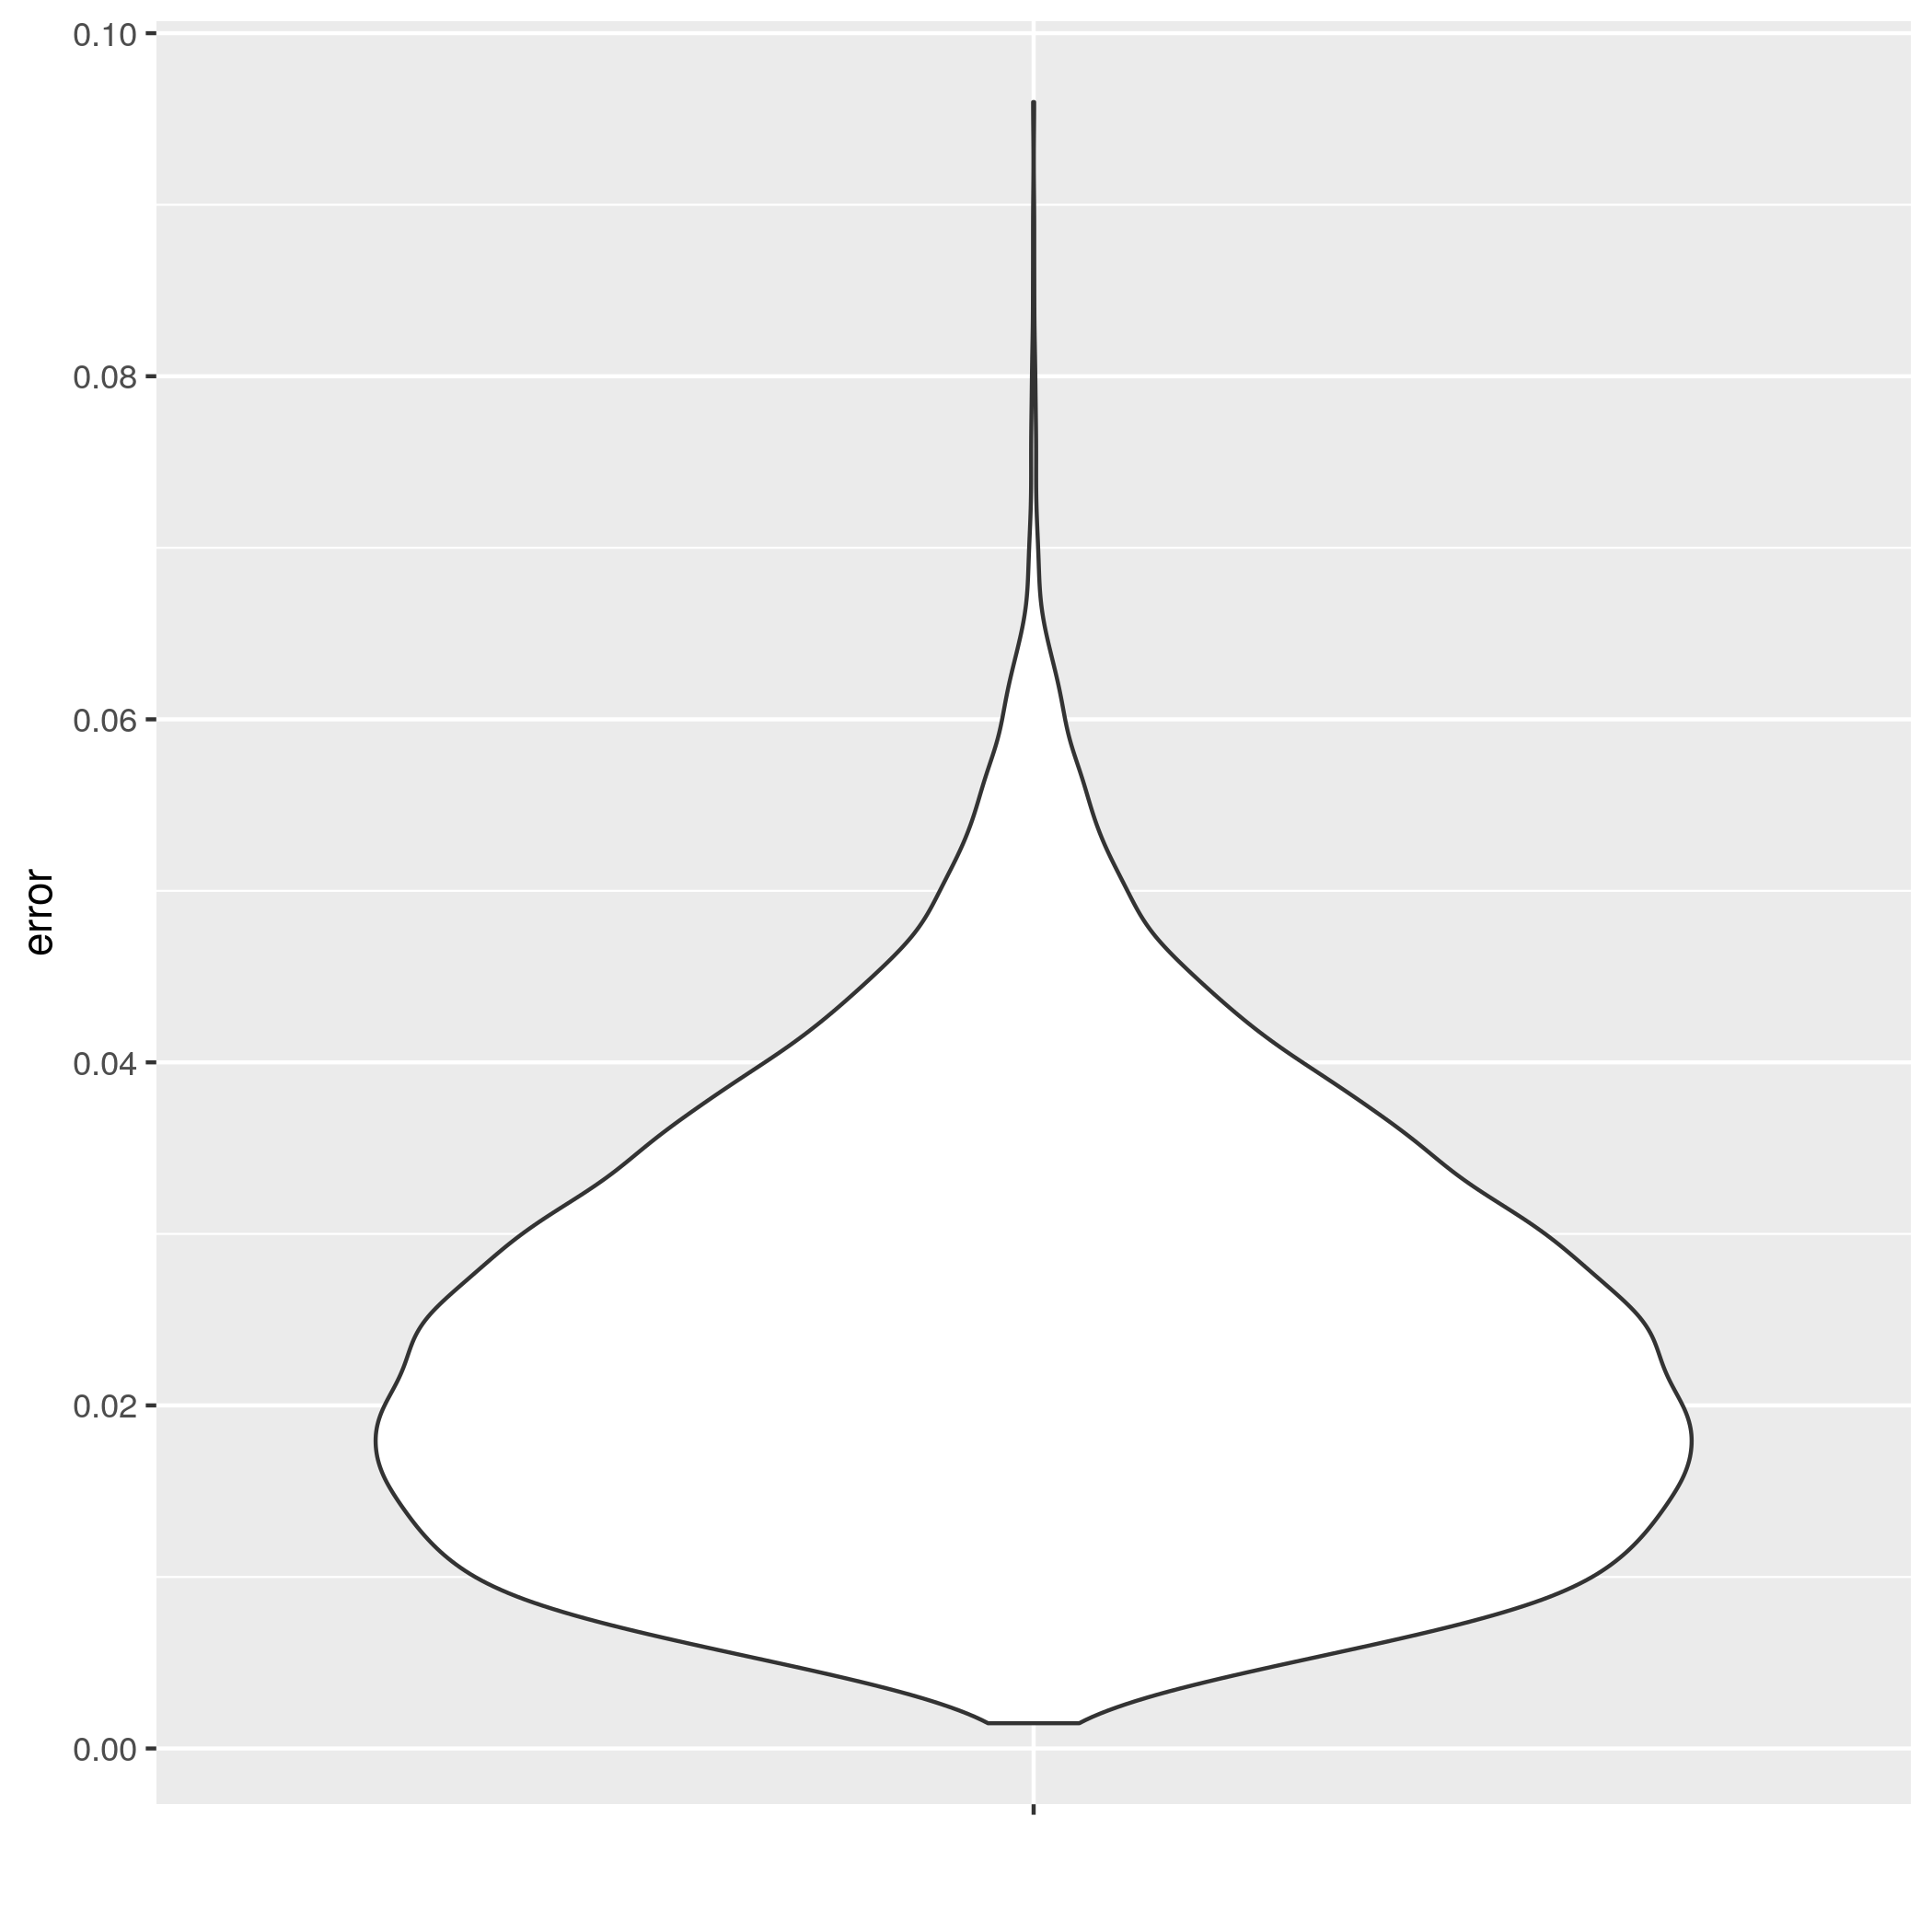
\includegraphics[height=0.3\textheight]{example_3/twin_error_violin_best.png}
    };   
    \path 
      (O) edge [anchor = south] node {} (A)
      (A) edge [anchor = south] node {} (B)
      (B) edge [anchor = south] node {} (CG)
      (CG) edge [anchor = south] node {} (DG)
      (B) edge [anchor = south east] node {} (CB)
      (CB) edge [anchor = south] node {} (DB)
      (A) edge [anchor = east] node {} (AT)
      (AT) edge [anchor = south] node {} (BT)
      (BT) edge [anchor = south east] node {} (CTG)
      (CTG) edge [anchor = south] node {} (DTG)
      (BT) edge [anchor = south] node {} (CTB)
      (CTB) edge [anchor = south] node {} (DTB)
    ; 
    \end{tikzpicture}
  }
  \label{fig:example_3_full_pipeline}
  \caption{Comparing to background noise: full pipeline}
\end{figure}
%%%%%%%%%%%%%%%%%%%%%%%%%%%%%%%%%%%%%%%%%%%%%%%%%%%%%%%%%%%%%%%%%%%%%%%%%%%%%%%%

\input{example_3/esses_gen.latex}

\input{example_3/esses_best.latex}

\input{example_3/esses_twin_gen.latex}

\input{example_3/esses_twin_best.latex}

\input{example_3/evidence_true.latex}

\input{example_3/evidence_twin.latex}
